% 3D Cone
% Author: Gene Ressler. Adapted to TikZ by Kjell Magne Fauske.
% See http://www.frontiernet.net/~eugene.ressler/ for more details.

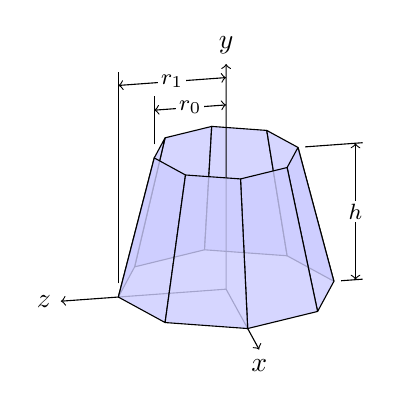
\begin{tikzpicture}[join=round]
    \tikzstyle{conefill} = [fill=blue!20,fill opacity=0.8]
    \tikzstyle{ann} = [fill=white,font=\footnotesize,inner sep=1pt]
    \tikzstyle{ghostfill} = [fill=white]
         \tikzstyle{ghostdraw} = [draw=black!50]
    \filldraw[conefill](-.775,1.922)--(-1.162,.283)--(-.274,.5)
                        --(-.183,2.067)--cycle;
    \filldraw[conefill](-.183,2.067)--(-.274,.5)--(.775,.424)
                        --(.516,2.016)--cycle;
    \filldraw[conefill](.516,2.016)--(.775,.424)--(1.369,.1)
                        --(.913,1.8)--cycle;
    \filldraw[conefill](-.913,1.667)--(-1.369,-.1)--(-1.162,.283)
                        --(-.775,1.922)--cycle;
    \draw(1.461,.107)--(1.734,.127);
    \draw[arrows=<->](1.643,1.853)--(1.643,.12);
    \filldraw[conefill](.913,1.8)--(1.369,.1)--(1.162,-.283)
                        --(.775,1.545)--cycle;
    \draw[arrows=->,line width=.4pt](.274,-.5)--(0,0)--(0,2.86);
    \draw[arrows=-,line width=.4pt](0,0)--(-1.369,-.1);
    \draw[arrows=->,line width=.4pt](-1.369,-.1)--(-2.1,-.153);
    \filldraw[conefill](-.516,1.45)--(-.775,-.424)--(-1.369,-.1)
                        --(-.913,1.667)--cycle;
    \draw(-1.369,.073)--(-1.369,2.76);
    \draw(1.004,1.807)--(1.734,1.86);
    \filldraw[conefill](.775,1.545)--(1.162,-.283)--(.274,-.5)
                        --(.183,1.4)--cycle;
    \draw[arrows=<->](0,2.34)--(-.913,2.273);
    \draw(-.913,1.84)--(-.913,2.447);
    \draw[arrows=<->](0,2.687)--(-1.369,2.587);
    \filldraw[conefill](.183,1.4)--(.274,-.5)--(-.775,-.424)
                        --(-.516,1.45)--cycle;
    \draw[arrows=<-,line width=.4pt](.42,-.767)--(.274,-.5);
    \node[ann] at (-.456,2.307) {$r_0$};
    \node[ann] at (-.685,2.637) {$r_1$};
    \node[ann] at (1.643,.987) {$h$};
    \path (.42,-.767) node[below] {$x$}
        (0,2.86) node[above] {$y$}
        (-2.1,-.153) node[left] {$z$};
\end{tikzpicture}